\interlude[1]{Hybridization}
\begin{frame}[light,s]{}
  \vspace{1cm}
  \large
  \vollkorn

  \begin{columns}[c]
    \begin{column}{.30\linewidth}
      % \vfill
      %  …that hybrid, practical, post-quantum cryptography is built by combining pre-quantum and post-quantum primitives.

      % \vfill
      %  …that key encapsulation methods can be combined, rendering a protocol like Rosenpass useful in pre-quantum as well
      %  as post-quantum settings.

      %  \vfill
      %  …why combining protocols like WireGuard and Rosenpass directly is still useful to enable code-reuse and to avoid
      %  loosing trust in established systems like WireGuard.
      %  \vfill
      In the following slides you will learn …
      \par\vspace{1.5em}
      … that hybrid security can be achieved by building hybrid primitives and that it is not always wise to do so.
    \end{column}

    \begin{column}{.40\linewidth}
      
\includegraphics[width=.7\linewidth,padding=-.2cm .2cm .2cm .2cm]{graphics/krapfen-prezel-bunny.pdf}
    \end{column}
  \end{columns}
\end{frame}

\begin{frame}{Combining two KEMs with the GHP Combiner}
  \begin{columns}[c]
    \begin{column}{.4\linewidth}
      \small
      \begin{itemize}
        \item \say{Giacon-Heuer-Poettering} \citeGhp
        \item Running both KEMs in parallel
        \item Secret keys, public keys, and ciphertexts are concatenated
        \item Shared keys are hashed together
        \item Ciphertexts included in hash for proof-related reasons
      \end{itemize}
    \end{column}

    \begin{column}{.6\linewidth}
      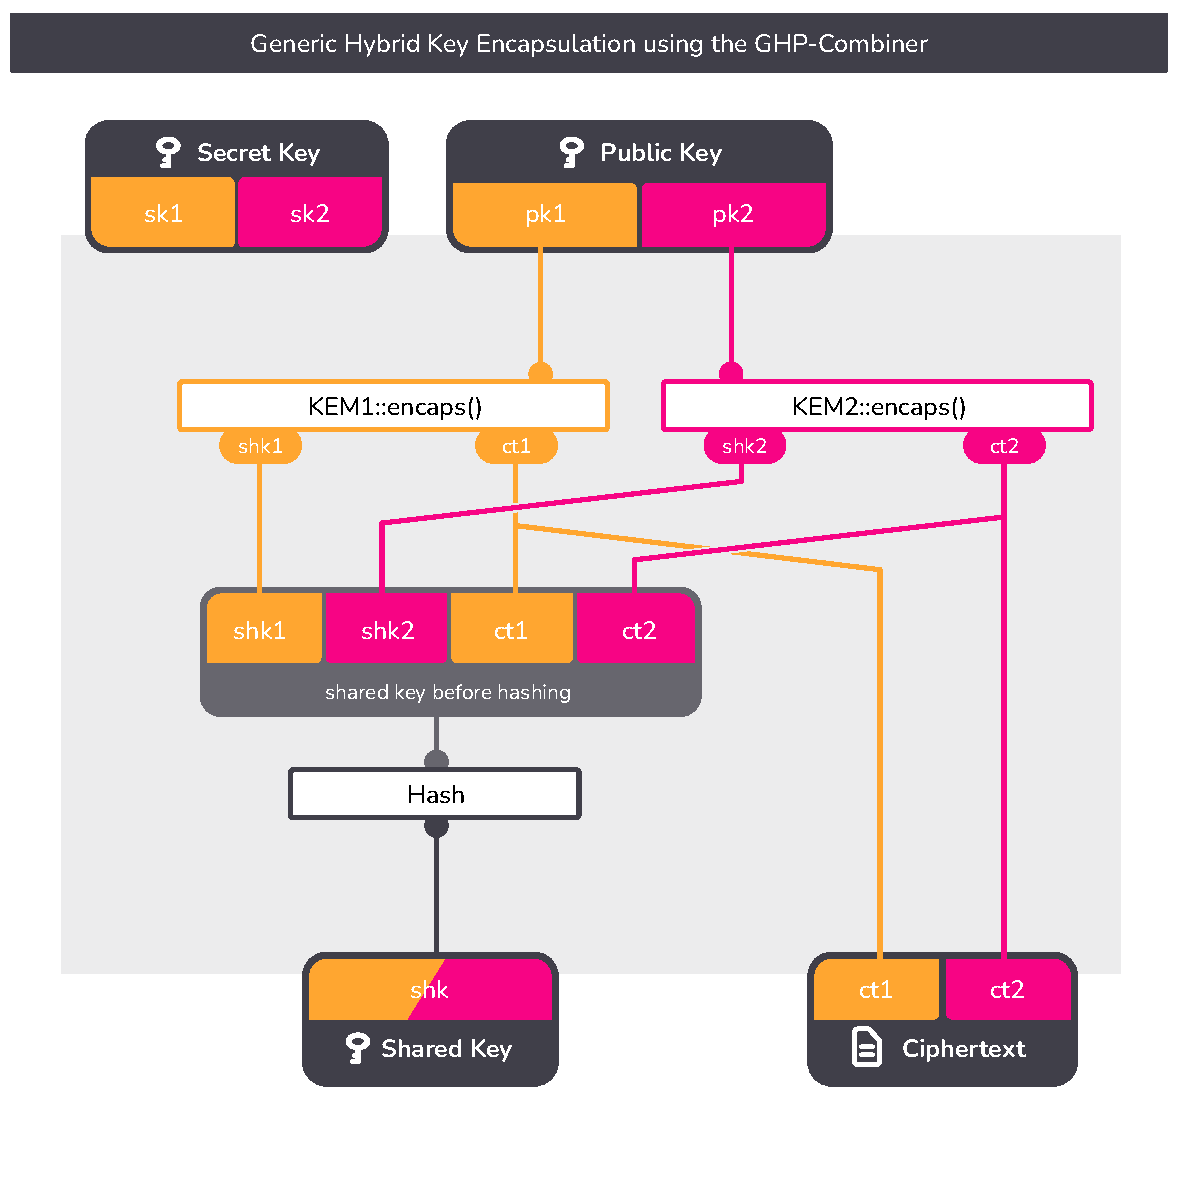
\includegraphics[height=.92\textheight,page=1,clip=true,trim={0.5cm 1cm 0.7cm 1.5cm}]{graphics/rosenpass-encapsulation-combiner.pdf}
    \end{column}

  \end{columns}
\end{frame}

\begin{frame}{Turning a NIKE into a KEM}
  \begin{columns}[c]
    \begin{column}{.6\linewidth}
      \includegraphics[height=.92\textheight,page=2,clip=true,trim={0.5cm 1cm 0.7cm 1.5cm}]{graphics/rosenpass-encapsulation-combiner.pdf}
    \end{column}

    \begin{column}{.4\linewidth}
      \small
      \begin{itemize}
        \item From the HPKE RFC \citeHpke
        \item \emph{Remote} keypair is static keypair
        \item \emph{Local} keypair is temporary keypair
        \item Local keypair public key is treated as ciphertext
        \item For proof-related reasons, ciphertext and public key
          are included in hash
        \item Work by Blanchet, Hauck, Kiltz, Lipp, Riepel
      \end{itemize}
    \end{column}
  \end{columns}
\end{frame}

\begin{frame}{X-Wing \citeXwing}
  \begin{columns}[c]
    \begin{column}{.4\linewidth}
      \small
      \begin{itemize}
        \item Combines ML-KEM and x25519
        \item Techniques from DHKEM to turn x25519 into a KEM
        \item Techniques from GHP to combine the two
        \item Optimizations applied to make hashing more efficient
        \item Bespoke proof of security
        \item Work by Borbosa, Connolly, Duarte, Schwabe, Varner, Westerbaan
      \end{itemize}
    \end{column}

    \begin{column}{.6\linewidth}
      \includegraphics[height=.92\textheight,page=3,clip=true,trim={0.5cm 1cm 0.7cm 1.5cm}]{graphics/rosenpass-encapsulation-combiner.pdf}
    \end{column}

  \end{columns}
\end{frame}

\begin{frame}{Rosenpass \& WireGuard Hybridization}
  \begin{columns}[c]

    \begin{column}{.6\linewidth}
      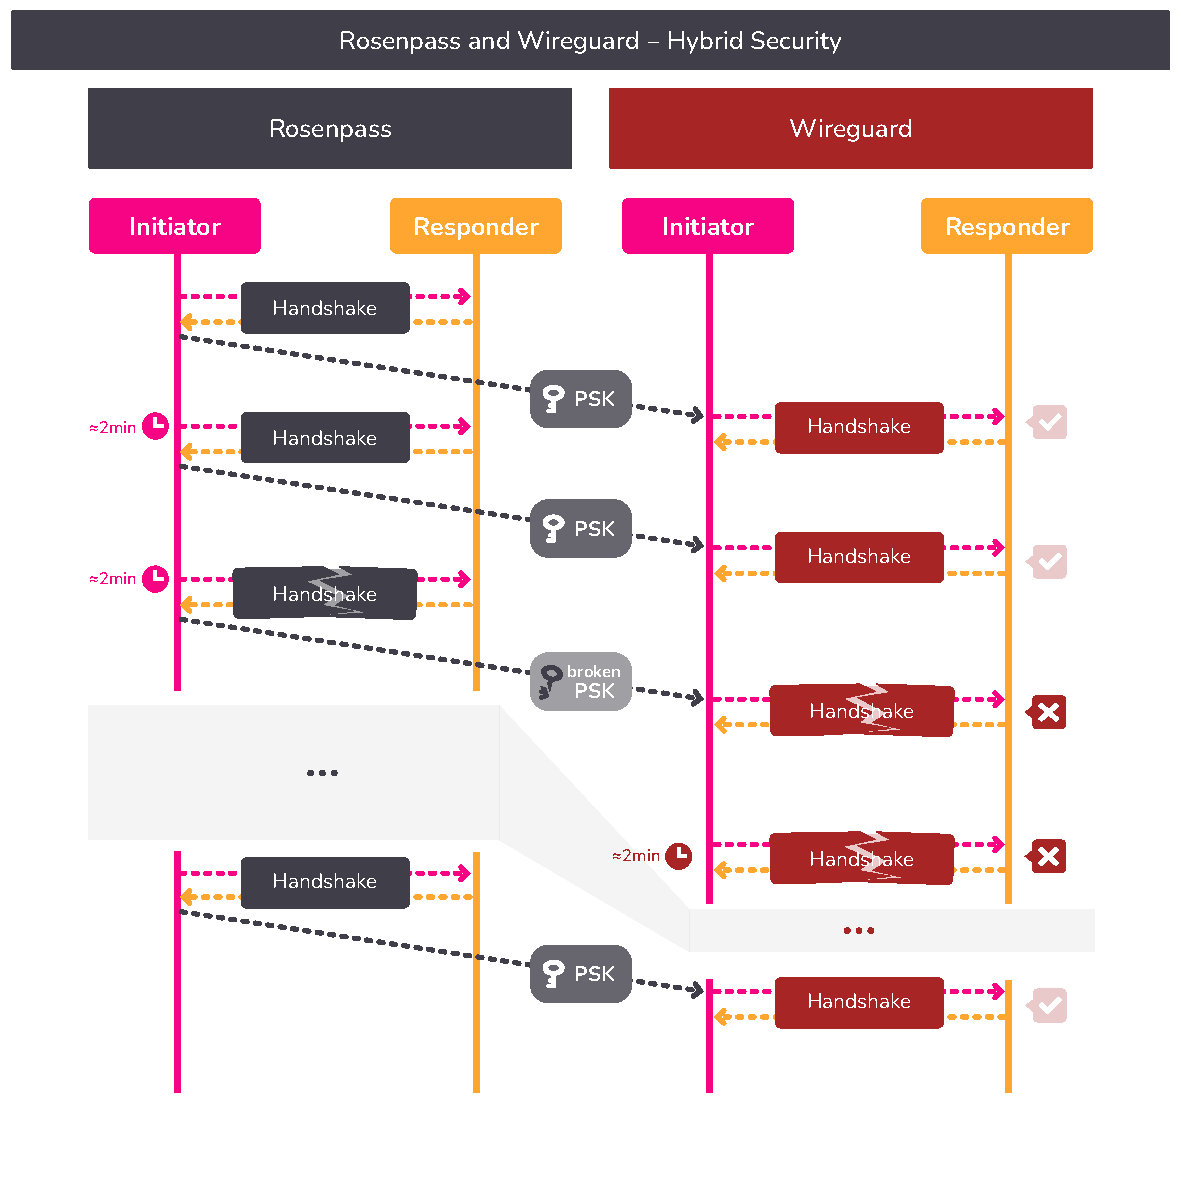
\includegraphics[height=\textheight, clip=true,trim=0cm .5cm 0cm 3.2cm,padding=-1cm 0cm 0cm 0cm]{graphics/rosenpass-wireguard-hybrid-security.pdf}
    \end{column}

    \begin{column}{.4\linewidth}
      \small
      \begin{itemize}
        \item Rosenpass and WireGuard are hybridized on the procol level
        \item Preserving efficiency of and trust in WireGuard
        \item Straightforward transition path; existing WireGuard implementation remains in use
        \item Key from Rosenpass used as PSK in WireGuard
      \end{itemize}
    \end{column}

  \end{columns}
\end{frame}
